%\subsubsection{Quark/Gluon jets uncertainty}
\label{subsec:bkg_uncer_qg}

Jet flavor response and composition uncertainties consider the different responses of quark- and gluon-initiated jets. 
The response uncertainties are centrally derived from dijet events, using alternative MC samples, specifically Pythia 8 and Herwig++. 
For flavor composition, uncertainties are typically assumed based on a presumed 50/50 quark/gluon mix, with a conservative approach that assumes 100\% uncertainty. However, in VBS topologies, which tend to be quark-enriched, these uncertainties can limit measurement sensitivity. 
To mitigate this, we analyze the gluon fraction within our analysis phase-space. This analysis allows us to rederive jet flavor-related uncertainties using custom gluon fractions, potentially reducing these uncertainties.

The estimation of the gluon fraction across various analysis regions and samples is performed as a function of the small-$R$ jet $\pt$ and $\eta$. This is achieved by utilizing truth parton label information in MC samples to discern the proportions of quarks and gluons. For the purpose of quark estimation, all jets except those initiated by b-quarks are considered in the denominator.

Two-dimensional histograms, representing the gluon fraction as a function of jet $\pt$ and $\eta$, serve as inputs for recalculating jet flavor and composition uncertainties. Each MC sample is associated with a single input file. The gluon fraction for a specific ($\pt$, $\eta$) bin is determined by aggregating data across all regions.

To account for the uncertainty in the gluon fraction, additional inputs are utilized. The uncertainty for a particular ($\pt$, $\eta$) bin, $\sigma_{gfrac}$, is calculated as follows:
\[
\sigma_{gfrac} = \sqrt{\sigma_{region}^{2} + \sigma_{gen}^{2}}
\]
Here, \(\sigma_{region}\) represents the maximal deviation in gluon fraction between the nominal and any analysis region. Meanwhile, \(\sigma_{gen}\) denotes the generator uncertainty, obtained from comparing alternative Pythia 8 and Herwig++ MC samples.

The inputs for the gluon fraction and their corresponding uncertainties in the \olep channel are illustrated in Figures \ref{fig:QGFracInputs2D1Lep} and \ref{fig:QGFracErrorInputs2D1Lep}, respectively. 
Comparison between old flavor uncertainties and newly derived flavor uncertainties is shown is Figure \ref{fig:1LepFlavorVarOldNew}. It is evident from this comparison that flavor composition uncertainties, in general, are reduced.

%%%%%%%%%%%%%


\begin{figure}[p]
    \centering
    \begin{subfigure}[b]{0.3\textwidth}
        \centering
        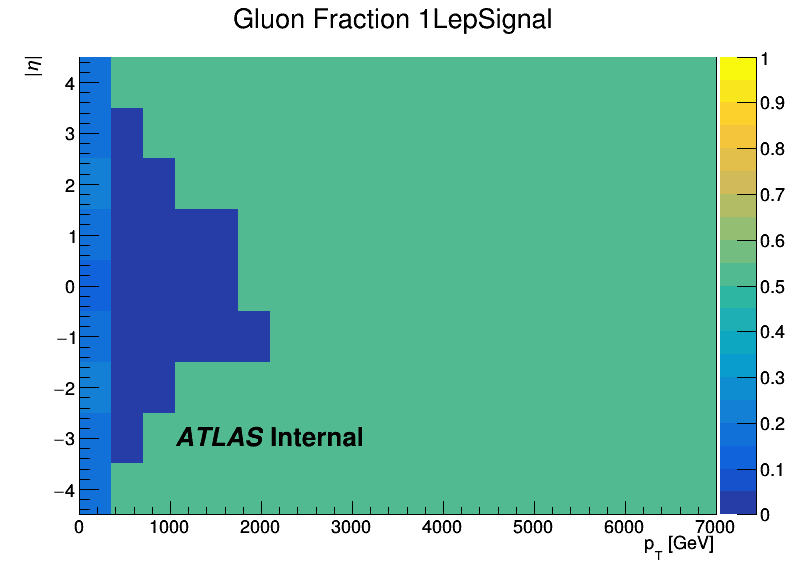
\includegraphics[width=\textwidth]{figures/QGfrac/GluonFrac2D_1LepSignal.png}
        \caption{Signal samples}
        \label{fig:GluonFracSignal}
    \end{subfigure}
    \hfill
    \begin{subfigure}[b]{0.3\textwidth}
        \centering
        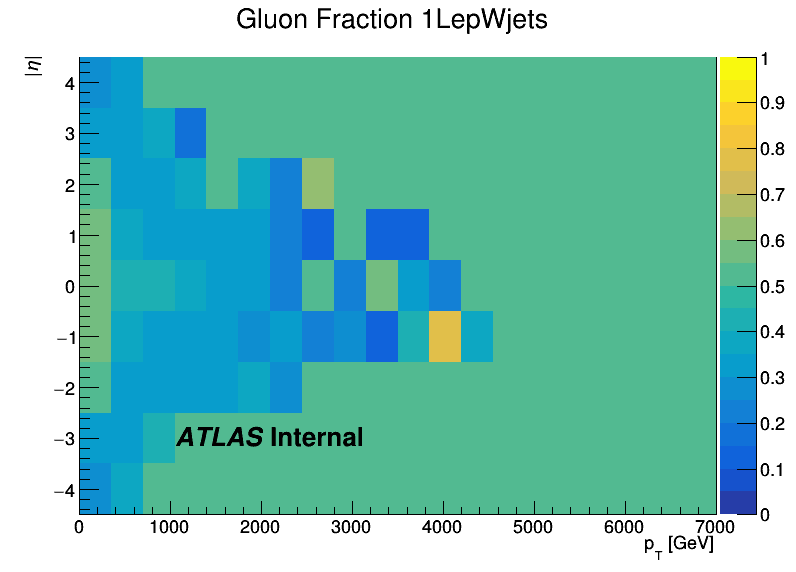
\includegraphics[width=\textwidth]{figures/QGfrac/GluonFrac2D_1LepWjets.png}
        \caption{\Wjets samples}
        \label{fig:GluonFracWjets}
    \end{subfigure}
    \hfill
    \begin{subfigure}[b]{0.3\textwidth}
        \centering
        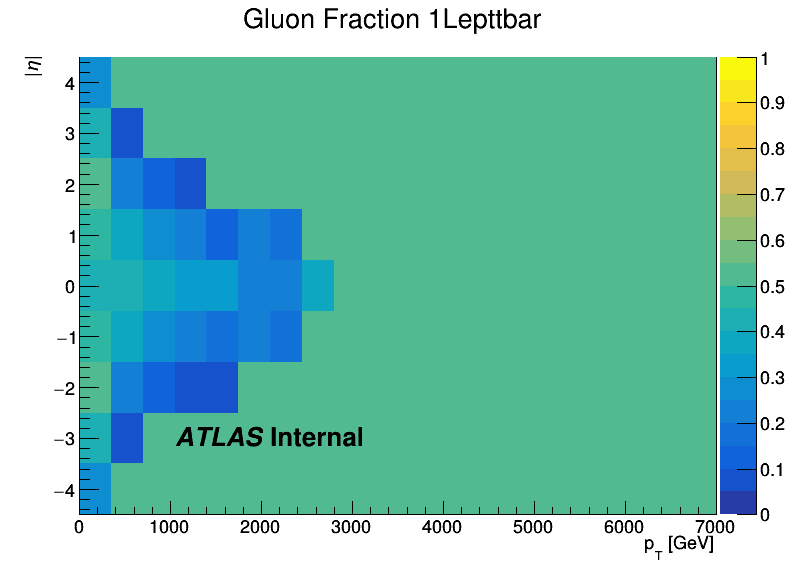
\includegraphics[width=\textwidth]{figures/QGfrac/GluonFrac2D_1Lepttbar.png}
        \caption{ttbar samples}
        \label{fig:GluonFracttbar}
    \end{subfigure}

    \bigskip

    \begin{subfigure}[b]{0.3\textwidth}
        \centering
        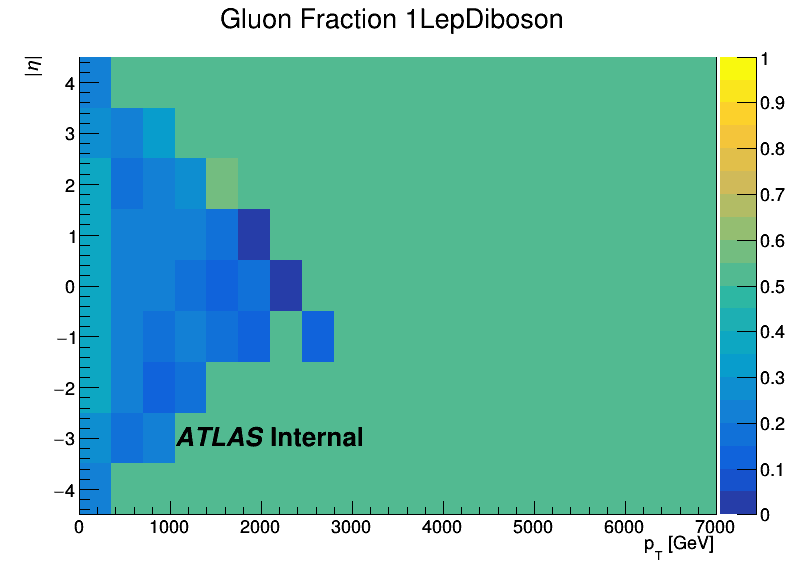
\includegraphics[width=\textwidth]{figures/QGfrac/GluonFrac2D_1LepDiboson.png}
        \caption{Diboson samples}
        \label{fig:GluonFracDiboson}
    \end{subfigure}
%    \hfill
    \begin{subfigure}[b]{0.3\textwidth}
        \centering
        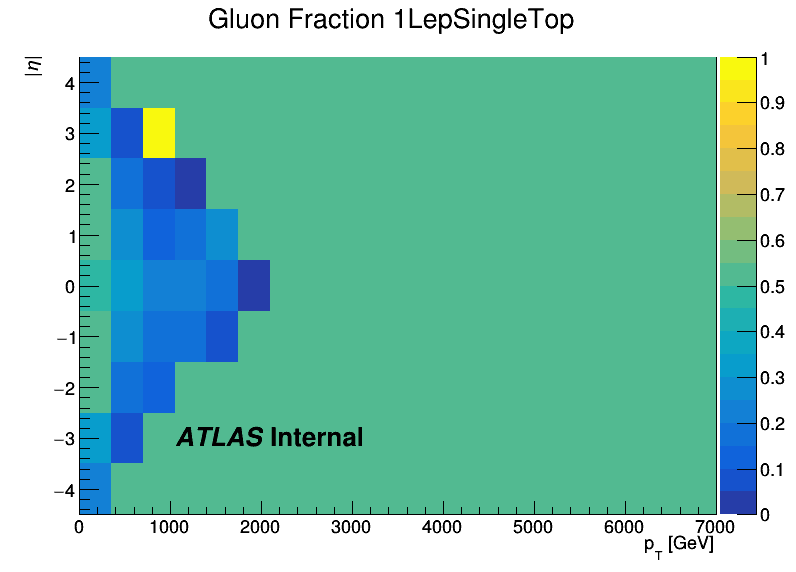
\includegraphics[width=\textwidth]{figures/QGfrac/GluonFrac2D_1LepSingleTop.png}
        \caption{Single top samples}
        \label{fig:GluonFracSingleTop}
    \end{subfigure}
    \hfill

    \caption{Gluon fraction inputs used to calculate jet uncertainties for the 1 lepton channel.}
    \label{fig:QGFracInputs2D1Lep}
\end{figure}


\begin{figure}[p]
    \centering
    \begin{subfigure}[b]{0.3\textwidth}
        \centering
        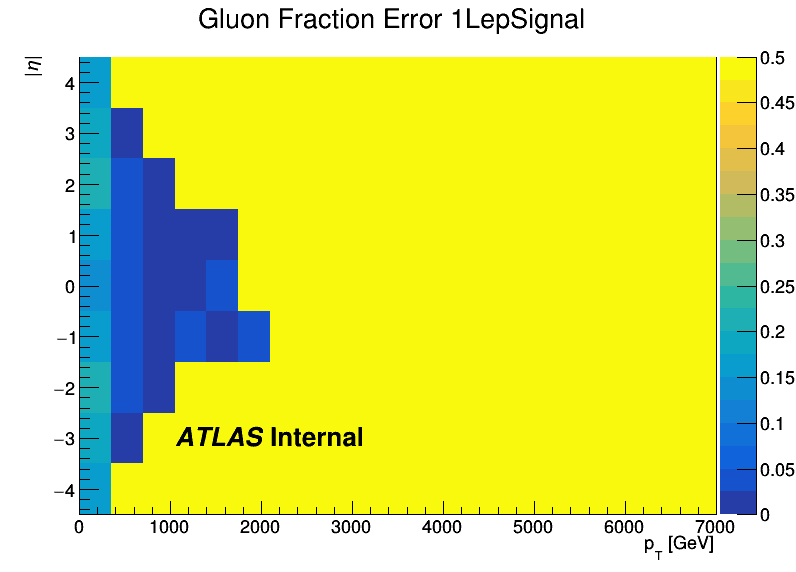
\includegraphics[width=\textwidth]{figures/QGfrac/GluonFracError2D_1LepSignal.png}
        \caption{Signal samples}
        \label{fig:GluonFracErrorSignal}
    \end{subfigure}
    \hfill
    \begin{subfigure}[b]{0.3\textwidth}
        \centering
        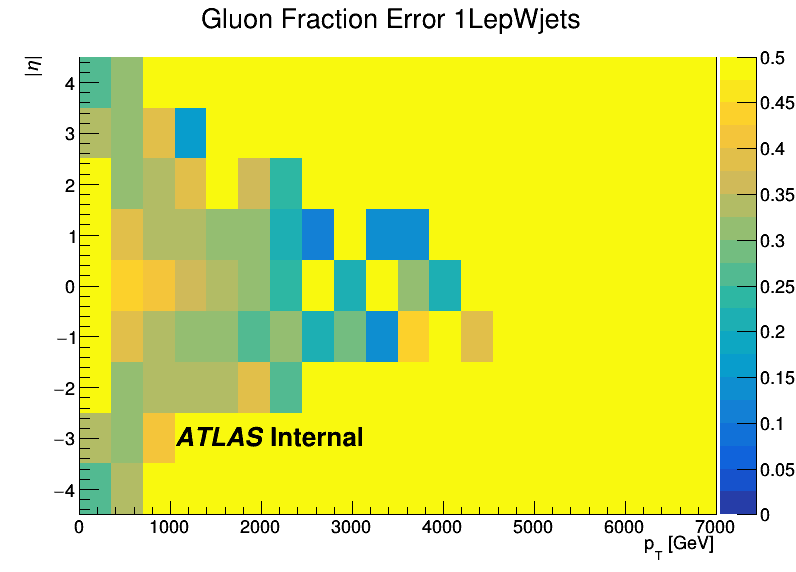
\includegraphics[width=\textwidth]{figures/QGfrac/GluonFracError2D_1LepWjets.png}
        \caption{\Wjets samples}
        \label{fig:GluonFracErrorWjets}
    \end{subfigure}
    \hfill
    \begin{subfigure}[b]{0.3\textwidth}
        \centering
        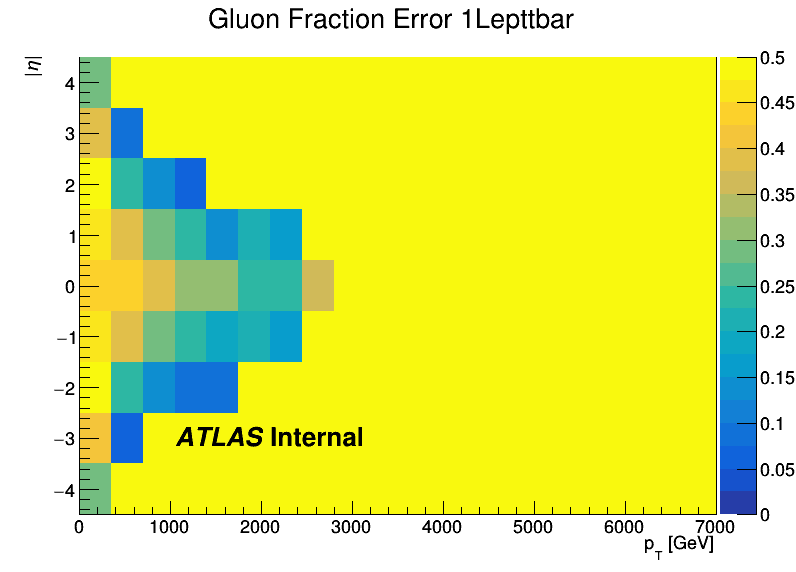
\includegraphics[width=\textwidth]{figures/QGfrac/GluonFracError2D_1Lepttbar.png}
        \caption{ttbar samples}
        \label{fig:GluonFracErrorttbar}
    \end{subfigure}

    \bigskip

    \begin{subfigure}[b]{0.3\textwidth}
        \centering
        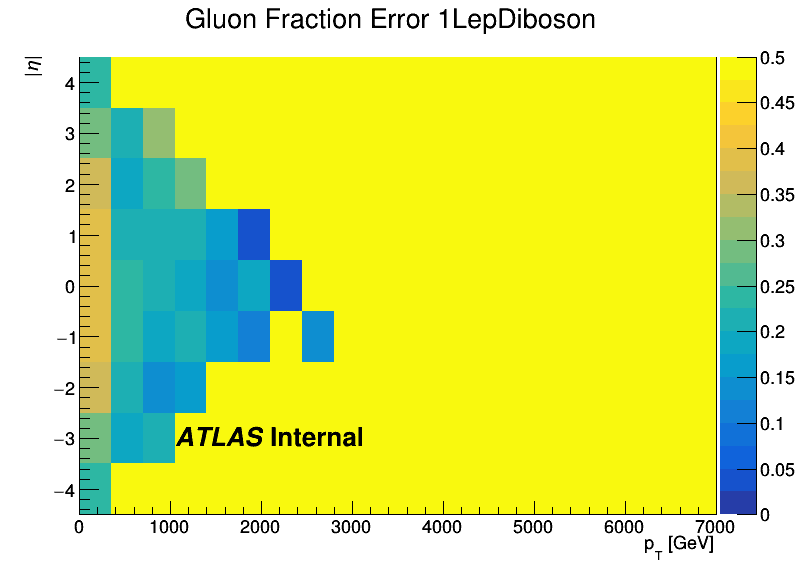
\includegraphics[width=\textwidth]{figures/QGfrac/GluonFracError2D_1LepDiboson.png}
        \caption{Diboson samples}
        \label{fig:GluonFracErrorDiboson}
    \end{subfigure}
%    \hfill
    \begin{subfigure}[b]{0.3\textwidth}
        \centering
        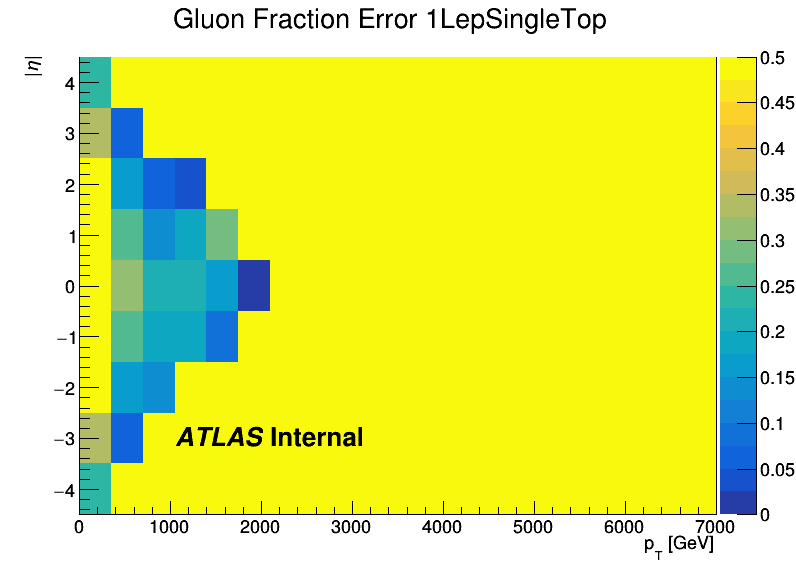
\includegraphics[width=\textwidth]{figures/QGfrac/GluonFracError2D_1LepSingleTop.png}
        \caption{Single top samples}
        \label{fig:GluonFracErrorSingleTop}
    \end{subfigure}
    \hfill

    \caption{Gluon fraction error inputs used to calculate jet uncertainties for the 1 lepton channel.}
    \label{fig:QGFracErrorInputs2D1Lep}
\end{figure}


\begin{figure}[ht]
    \centering
    \begin{subfigure}[b]{0.4\textwidth}
        \centering
        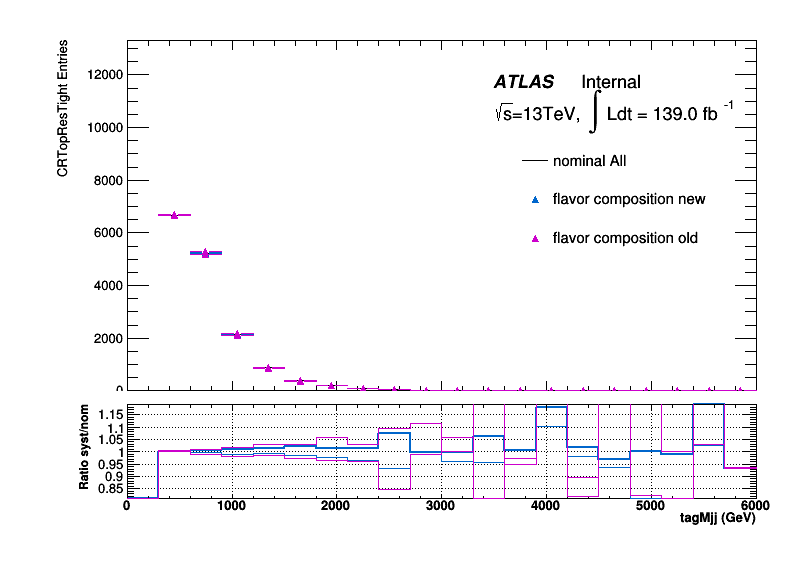
\includegraphics[width=\textwidth]{figures/1lep/FlavorVar/SystFCompCRTopResTight_All_tagMjj.png}
        \caption{Resolved TopCR Flavour Composition}
        \label{fig:ResolvedTopCRFlavourComposition}
    \end{subfigure}
    \quad % This adds some spacing between the figures in the same row
    \begin{subfigure}[b]{0.4\textwidth}
        \centering
        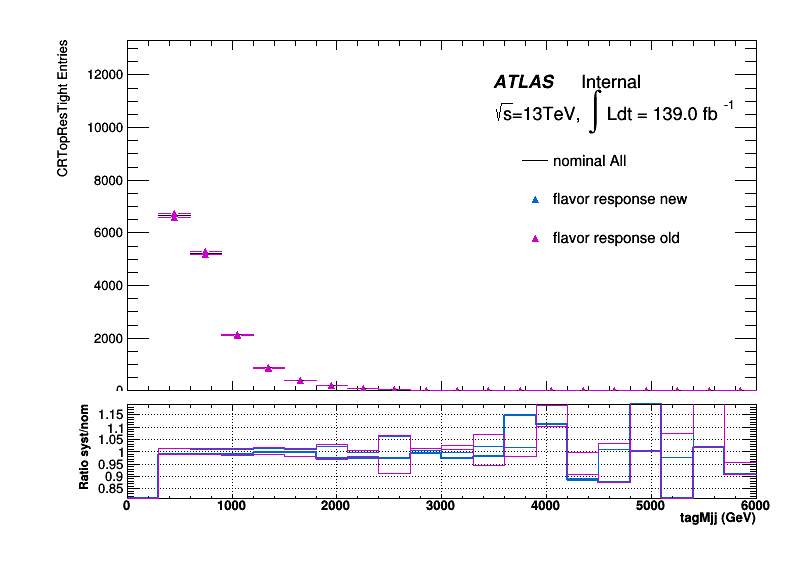
\includegraphics[width=\textwidth]{figures/1lep/FlavorVar/SystFResCRTopResTight_All_tagMjj.png}
        \caption{Resolved TopCR Flavour Response}
        \label{fig:ResolvedTopCRFlavourResponse}
    \end{subfigure}

    \bigskip % This adds extra vertical spacing between the rows of figures

    \begin{subfigure}[b]{0.4\textwidth}
        \centering
        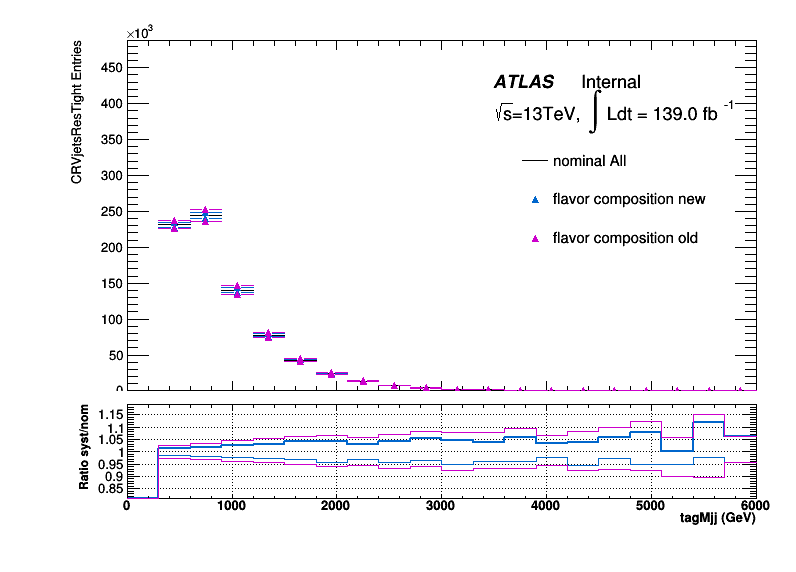
\includegraphics[width=\textwidth]{figures/1lep/FlavorVar/SystFCompCRVjetsResTight_All_tagMjj.png}
        \caption{Resolved WjetsCR Flavour Composition}
        \label{fig:ResolvedWjetsCRFlavourComposition}
    \end{subfigure}
    \quad % This adds some spacing between the figures in the same row
    \begin{subfigure}[b]{0.4\textwidth}
        \centering
        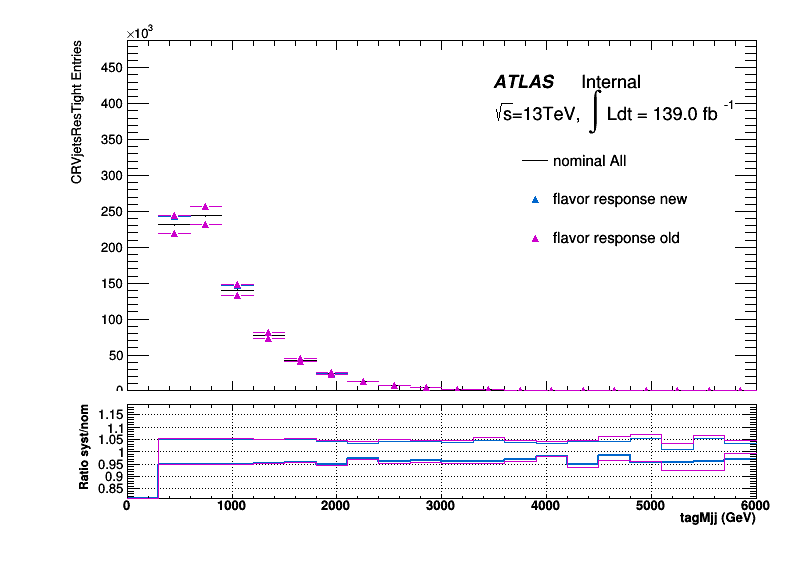
\includegraphics[width=\textwidth]{figures/1lep/FlavorVar/SystFResCRVjetsResTight_All_tagMjj.png}
        \caption{Resolved WjetsCR Flavour Response}
        \label{fig:ResolvedWjetsCRFlavourResponse}
    \end{subfigure}

    \caption{Comparison between old flavor uncertainties and newly derived flavor uncertainties.}
    \label{fig:1LepFlavorVarOldNew}
\end{figure}
